%Fiquemos com Deus e Nossa Senhora!
%Sao Jose de Cupertino rogai por nos!!
%Honra teu pai e tua mãe!
% ### Uses XeLaTeX ### %
% ### Needs beamer-master ### %
\documentclass[aspectratio=169]{beamer} %. Aspect Ratio 16:9

\usetheme{AI2} % beamerthemeSprace.sty
\usepackage[portuguese]{babel}
\usepackage[utf8]{inputenc}
\usepackage[T1]{fontenc}
\usepackage{ragged2e,gensymb}
\usepackage{amsmath,bm}

\DeclareMathOperator*{\argmin}{arg\,min}
\DeclareMathOperator*{\argmax}{arg\,max}
\DeclareMathOperator{\sign}{sgn}

% DATA FOR FOOTER
\date{2021}
\title{- Máquinas de Boltzmann Restritas}
\author{João Paulo Papa}
\institute{Advanced Institute for Artificial Intelligence (AI2)}

\begin{document}
% ####################################
% FIRST SLIDE 						:: \SliTit{This is the Title of the Talk}{A. B. Name}{Sprace}
% SUB-TITLE SLIDE 					:: \SliSubTit{<title>}{<explanation}
% SUB-SUB-TITLE SLIDE				:: \SliSubSubTit{<title>}{<explanation}
% SLIDE WITH TITLE 					:: \SliT{Title}{Content}
% SLIDE NO TITLE 						:: \Sli{Content} 
% SLIDE DOUBLE COLUMN WITH TITLE 	:: \SliDT{Title}{First Column}{Second Column}
% SLIDE DOUBLE COLUMN NO TITLE 		:: \SliD{First Column}{Second Column}
% SLIDE ADVANCED WITH TITLE 			:: \SliAdvT{Title}{Content}
% SLIDE ADVANCED NO TITLE 			:: \SliAdv{Content}
% SLIDE ADVANCED DOUBLE WITH TITLE 	:: \SliAdvDT{Title}{First Column}{Second Column}
% SLIDE ADVANCED DOUBLE NO TITLE 	:: \SliAdvD{First Column}{Second Column}
% SLIDE BLACK						:: \Black{ <Content> }
% SLIDE WHITE						:: \White{ <Content> }
% ITEMIZATION 						:: \begin{itemize}  \iOn{First} \iTw {Second} \iTh{Third} \end{itemize}
% COMMENT TEXT				 		:: \note{<comment>}
% SECTION 							:: \secx{Section} | \secxx{Sub-Section}
% BOLD SPRACE COLOR				:: \bfs{<text>}
% TABLE OF CONTENT					:: \tocitem{<title>}{<content>}
% LEFT ALIGN EQUATION				:: \begin{flalign*}  & <equation> &   \end{flalign*}
% CENTER ALIGN EQUATION	S			:: \begin{gather*} <equations>  \end{gather*}
% SLASH								:: \slashed{<>}
% BAR								:: \barr{<letter>} instead of \bar{<letter>}
% THEREFORE						:: use \portanto (larger and bold}
% 2 or 3 MATH SYMBOLS				:: \overset{<up>}{<down>} &  \underset{<below>}{\overset{<above>}{<middle>}}  
% INSERT TEXT IN FORMULA			:: \ins{<text>}
% EXERCISE							:: \exe{<exercise #>}{<exercise text>}
% SUGGESTED READING BOX			:: \sug{<references>}
% CITATION							:: \cittex{<citation>}
% CITATION DOUBLE COLUMN 			:: \cittexD{<citation>}
% TEXT POSITION						:: \texpos{<Xcm>}{<Ycm>}{<text>} origin = center of slide : x right | y down
% REFERENCE AT BOTTOM  S/D SLIDE		:: \refbotS{<reference>} \refbotD{<reference>}
% HIDDEN SLIDE						:: \hid
% COLOR BOX 						:: \blu{blue} + \red{rec} + \yel{yellow} + \gre{green} + \bege{beige}
% FRAME 							:: \fra{sprace} \frab{blue} \frar{red} + \fray{yellow} + \frag{green}		
% FIGURE 							:: \img{X}{Y}{<scale>}{Figure.png} 
% FIGURE							:: \includegraphics[scale=<scale>]{Figures/.png}
% FIGURE DOUBLE SLIDE NO TITLE		::  \img{-4}{0.5}{<scale>}{Figure.png} % Image 1st half
%									::  \img{4}{0.5}{<scale>}{Figure.png} % Image 2nd half
% FIGURE DOUBLE SLIDE WITH TITLE		::  \img{-4}{0}{<scale>}{Figure.png} % Image 1st half
%									::  \img{4}{0}{<scale>}{Figure.png} % Image 2nd half
% INCLUDING SWF (Flash)				:: \usepackage{media9} and \includemedia >> USE ACROBAT <<
%%%%%%%%%%%%%%%%%%%%%%%%%%%%%%%%%%%%%%%%%%%%%%%%%%
% ###############################################################################
% FIRST SLIDE
\SliTit{{\LARGE Máquinas de Boltzmann Restritas}}{Advanced Institute for Artificial Intelligence -- AI2}{https://advancedinstitute.ai}
%%%%%%%%%%%%%%%%%%%%%%%%%%%%%%%%%%%%%%%%%%%%%%%%%%
% ###############################################################################
% SLIDE SUB-TITLE
%\SliSubTit{Sub-Title}{Description}{}
%%%%%%%%%%%%%%%%%%%%%%%%%%%%%%%%%%%%%%%%%%%%%%%%%%
% ###############################################################################
%\SliSubSubTit{Sub-Sub-Title}{Description}
 %%%%%%%%%%%%%%%%%%%%%%%%%%%%%%%%%%%%%%%%%%%%%%%%%%


\SliT{Introdução}{

\justifying As Máquinas de Boltzmann Restritas, do inglês \emph{Restricted Boltzmann Machines} (RBMs) são técnicas baseadas no aprendizado de modelos de \textbf{energia}. Elas podem atuar nas etapas de:

\begin{itemize}
	\item Redução de dimensionalidade.
	\item Aprendizado de características.
	\item Classificação.
	\item Pré-treinamento de redes neurais MLP.
\end{itemize}

}

\Sli{
\justifying RBMs, de maneira geral, são modelos probabilísticos compostos por duas camadas: visível $\bm{v}\in\{0,1\}^m$ (entrada) e escondida $\bm{h}\in\{0,1\}^n$. Enquanto que a camada visível é responsável pela leitura dos dados, a camada escondida mapeia sua distribuição por meio de unidades escondidas (binárias, inicialmente) $h_j$ e uma matriz de peso $\bm{W}\in\mathbb{R}^{m\times n}$ que conecta essas duas camadas. Adicionalmente, temos as camadas de bias $\bm{a}\in\mathbb{R}^m$ e $\bm{b}\in\mathbb{R}^n$ conectadas às camadas visível e escondida, respectivamente.

\begin{figure}[htb]
   \centering
	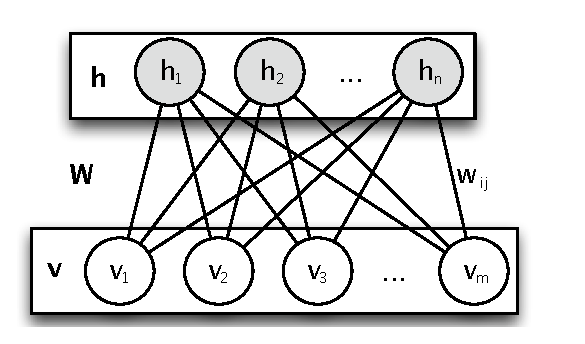
\includegraphics[scale=0.47]{figs/rbm.eps}
\end{figure}
}

\Sli{
A \textbf{energia} de uma RBM é dada por:
\begin{equation}
E(\textbf{v},\textbf{h})=-\sum_{i=1}^m\sum_{j=1}^nv_ih_jw_{ij}-\sum_{i=1}^ma_iv_i-\sum_{j=1}^nb_jh_j,
\end{equation}
em que a probabilidade de uma dada configuração $(\textbf{v},\textbf{h})$ é calculada como segue:
\begin{equation}
P(\textbf{v},\textbf{h})=\frac{e^{-E(\textbf{v},\textbf{h})}}{Z},
\end{equation}
onde $Z$ denota a chamada \textbf{constante de normalização/função de partição}, a qual pode ser calculada da seguinte forma:
\begin{equation}
Z=\sum_{\textbf{v},\textbf{h}}e^{-E(\textbf{v},\textbf{h})}.
\end{equation}
}

\Sli{
\justifying A probabilidade de uma amostra do conjunto de dados $\bm{v}$ (unidade visível) é definida como segue:
\begin{equation}
\label{e.probability}
P(\textbf{v})=\sum_{\textbf{h}}P(\textbf{v},\textbf{h})=\frac{\sum_{\textbf{h}}e^{-E(\textbf{v},\textbf{h})}}{Z}.
\end{equation}

\justifying Seja ${\cal X}=\{\bm{x}_1,\bm{x}_2,\ldots,\bm{x}_z\}$ um conjunto de treinamento. A etapa de aprendizado de uma RBM, de maneira geral, objetiva diminuir a energia de cada amostra de treinamento $\bm{x}_i$ visando aumentar a sua probabilidade no conjunto.

\begin{figure}[htb]
   \centering
	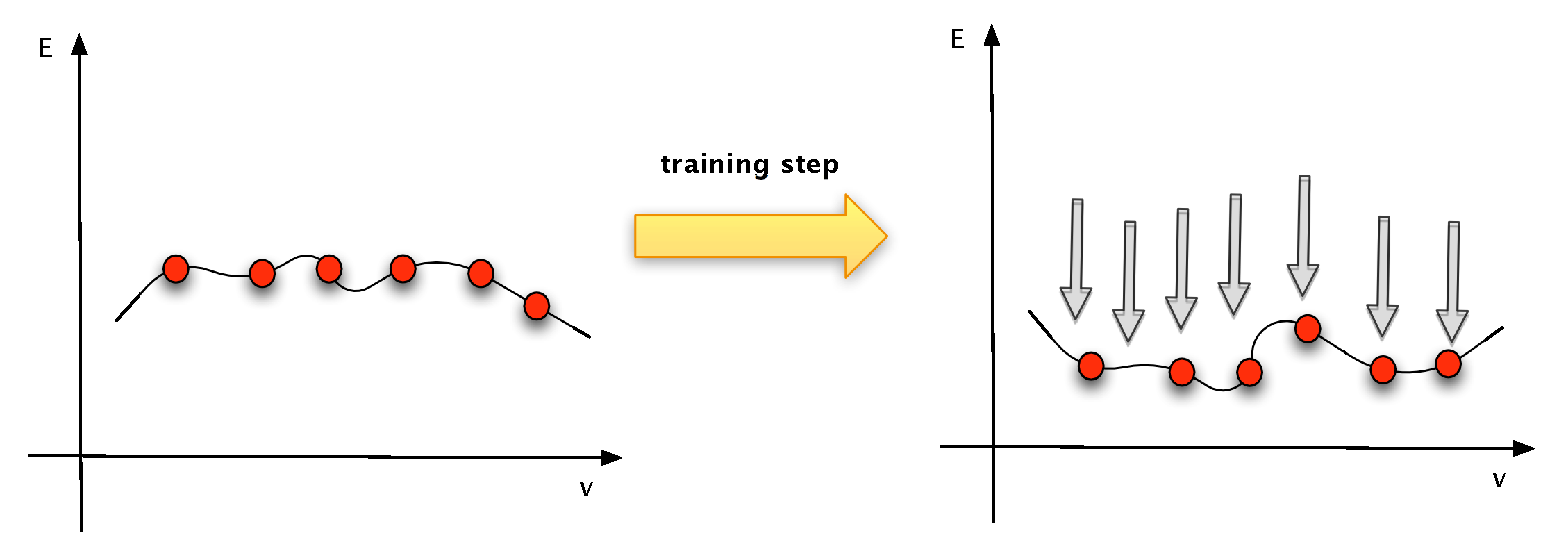
\includegraphics[scale=0.33]{figs/training_step.eps}
\end{figure}
}

\Sli{
\justifying A verossimilhança do conjunto de dados considerando apenas uma amostra de treinamento $\bm{v}\leftarrow\bm{x}\in{\cal X}$ é calculada como segue:
\begin{equation}
\phi=\log P(\textbf{v})=\phi^+-\phi^-,
\end{equation}
em que
\begin{equation}
\phi^+=\log \sum_{\textbf{h}}e^{-E(\textbf{v},\textbf{h})}
\end{equation}
e
\begin{equation}
\phi^-=\log Z=\log \sum_{\textbf{v},\textbf{h}}e^{-E(\textbf{v},\textbf{h})}.
\end{equation}
Agora, a questão é: Como podemos treinar uma RBM?
}

\Sli{

\justifying Basicamente, a etapa de treinamento consiste em atualizar o conjunto de pesos $\bm{W}$ no sentido de maximizar o logaritmo da verossimilhança do conjunto de dados de treinamento até algum critério de convergência ter sido atingido. Usualmente, utilizamos o gradiente descendente estocástico para tal propósito:

\begin{equation}
\textbf{W}^{t+1}\leftarrow \textbf{W}^t+\eta\left(\frac{\partial \phi^+}{\partial \textbf{W}}-\frac{\partial \phi^-}{\partial \textbf{W}}\right),
\end{equation}
em que o \textbf{gradiente positivo} é dado por (fácil de ser calculado):
\begin{equation}
\label{e.positive_gradient}
\frac{\partial \phi^+}{\partial \textbf{W}}=\textbf{v}^TP(\textbf{h}|\textbf{v}).
\end{equation}
}

\Sli{
\justifying O lado direito da Equação 9 pode ser calculado como segue:
\begin{equation}
\label{e.probh}
P(\textbf{h}|\textbf{v})=\prod_{j=1}^nP(h_j=1|\textbf{v}),
\end{equation}
e
\begin{equation}
P(h_j=1|\textbf{v})=\sigma\left(\sum_{i=1}^mw_{ij}v_i+b_j\right).
\end{equation}
Neste caso, $\sigma(c)=1/(1+\exp(-c))$. 
}

\Sli{
\justifying Entretanto, o grande problema consiste no \textbf{gradiente negativo}, o qual é dado por:
\begin{equation}
\frac{\partial \phi^-}{\partial \textbf{W}}= \textbf{v}^TP(\textbf{v}|\textbf{h}),
\end{equation}
em que $\textbf{v}$ denota a estimativa (model) dos dados de entrada $\textbf{v}$, e $P(\textbf{v}|\textbf{h})$ é dado por:
\begin{equation}
P(\textbf{v}|\textbf{h})=\prod_{i=1}^mP(v_i=1|\textbf{h}),
\end{equation}
e
\begin{equation}
\label{e.probv}
P(v_i=1|\textbf{h})=\sigma\left(\sum_{j=1}^nw_{ij}h_j+a_i\right).
\end{equation}
O problema é obter uma boa aproximação do modelos, ou seja, $\frac{\partial \phi^-}{\partial \textbf{W}}$, o qual requer um grande número de iterações.
}

\Sli{
\justifying Usualmente, podemos modelar a tarefa de estimar a probabilidade condicional por meio de uma Cadeia de Markov, do inglês \emph{Markov Chain Monte Carlo} (MCMC), a qual modela cada passo na direção da aproximação do dados reais como sendo uma cadeia de Markov.\newline

\justifying Uma cadeia de Markov é, basicamente, um grafo direcionado e ponderado que obedece algumas propriedades (Teorema Ergódico):
\begin{figure}[htb]
   \centering
	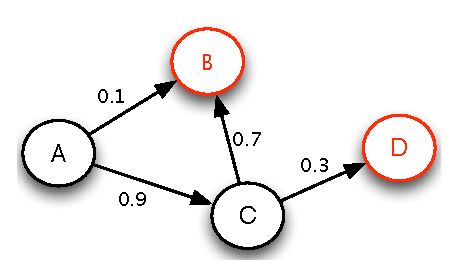
\includegraphics[scale=0.67]{figs/markov_chain.eps}
\end{figure}
}

\Sli{
\justifying Uma das abordagens mais famosas para amostragem em cadeias de Markov é a conhecida por \textbf{amostragem de Gibbs}, a qual aproxima a solução da verossimilhança quando $k\rightarrow \infty$, em que $k$ corresponde ao número de iterações.

\begin{figure}[htb]
   \centering
	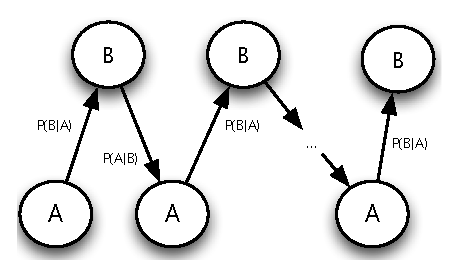
\includegraphics[scale=0.77]{figs/markov_gibbs.eps}
\end{figure}
}

\Sli{
\justifying Como podemos utilizar a amostragem de Gibbs para treinar RBMs? Suponha que tenhamos uma cadeia de Markov ${\cal C}=\{\textbf{v},\tilde{\textbf{v}}^1,\tilde{\textbf{v}}^2,\dots,\tilde{\textbf{v}}^k\}$ composta pelo dado de entrada (estado inicial) $\textbf{v}$ e sua reconstrução no tempo $t$ dada por $\tilde{\textbf{v}}^t$.

\begin{figure}[htb]
   \centering
	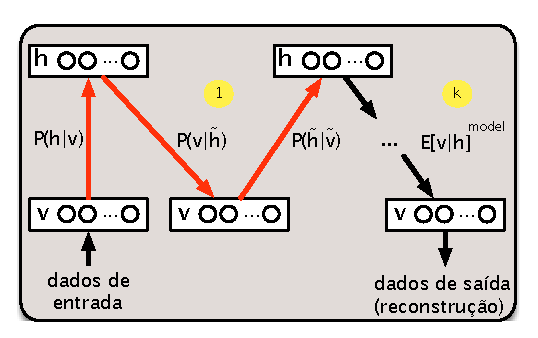
\includegraphics[scale=0.73]{figs/gibbs.eps}
\end{figure}
Problema? Alto custo computacional dado que precisamos de $k\rightarrow \infty$ para uma boa aproximação do modelo.
}

\Sli{
\justifying Hinton (2002)\footnote{Hinton, G. E. ``Training products of experts by minimizing contrastive divergence", \emph{Neural Computation}, 14(8), 1771-1800, 2002.} propuseram a Divergência Contrastiva, do inglês \emph{Contrasttive Divergence} (CD), a qual é uma alternativa mais eficiente à amostragem de Gibbs.

\begin{figure}[htb]
   \centering
	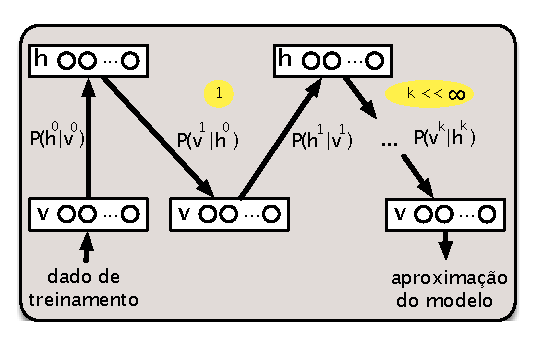
\includegraphics[scale=0.57]{figs/cd.eps}
\end{figure}
Usualmente, $k=1$. Problema? Modelos estimados tendem a se tornar muito parecidos com as amostras de treinamento.
}

\Sli{
\justifying Posteriormente, novos parâmetros foram introduzidos para melhorar o processo de treinamento: decaimento de peso $\lambda$ e momento $\alpha$. Desta forma, temos novas equações de atualização:

\begin{equation}
\label{e.updateW2}
 \textbf{W}^{t+1}=\textbf{W}^t+\underbrace{\eta(P(\textbf{h}|\textbf{v})\textbf{v}^T-P(\tilde{\textbf{h}}|\tilde{\textbf{v}})\tilde{\textbf{v}}^T)-\lambda\textbf{W}^T+\alpha\Delta\textbf{W}^{t-1}}_{=\Delta\textbf{W}^t},
\end{equation}

\begin{equation}
\label{e.updatea2}
\textbf{a}^{t+1}=\textbf{a}^t+\underbrace{\eta(\textbf{v}-\tilde{\textbf{v}})+\alpha\Delta \textbf{a}^{t-1}}_{=\Delta\textbf{a}^t}
\end{equation}
e

\begin{equation}
\label{e.updateb2}
\textbf{b}^{t+1}=\textbf{b}^t+\underbrace{\eta(P(\textbf{h}|\textbf{v})-P(\tilde{\textbf{h}}|\tilde{\textbf{v}}))+\alpha\Delta \textbf{b}^{t-1}}_{=\Delta\textbf{b}^t}.
\end{equation}
}

\Sli{
\justifying A seguir, mostraremos um exemplo do uso de uma RBM para reconstrução de imagens binárias. O critério de minimização foi o do erro médio quadrático, do inglês \emph{Mean Squared Error} (MSE), entre os pixels da imagem de entrada e da imagem reconstruída. A base de dados a ser adotada é a MNIST, que consiste em imagens de dígitos manuscritos.

\begin{figure}[!ht]
  \centerline{\begin{tabular}{cc}
      	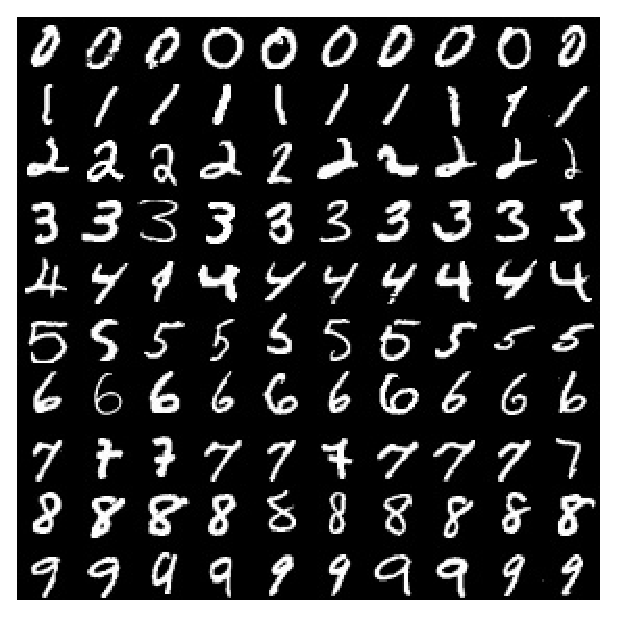
\includegraphics[width=3.1cm,height=3.1cm]{./figs/mosaic_MNdist_dataset.eps} &
      	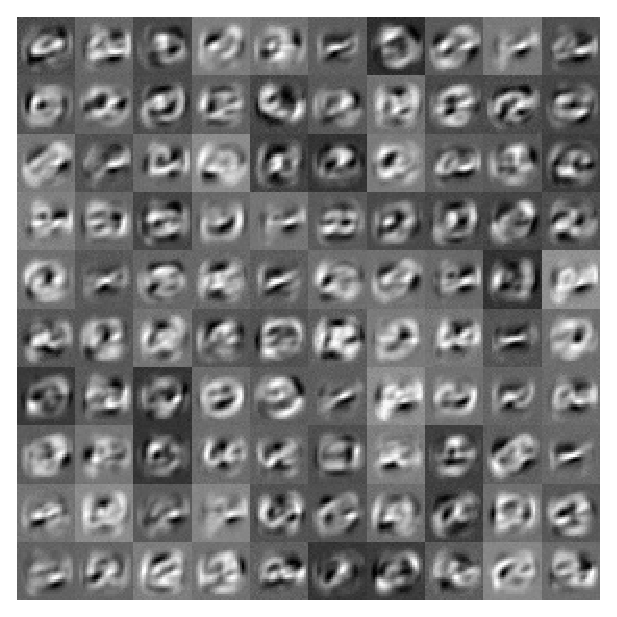
\includegraphics[width=3.1cm,height=3.1cm]{./figs/mosaicMNIST_weights.eps} \\
      	(a) & (b)
\end{tabular}}
\caption{Exemplos de imagens base MNIST: (a) imagens originais e (b) imagens dos pesos da rede.}
\label{f.datasets}
\end{figure}
}

\Sli{
Exemplo de uma RBM treinada apenas com dígitos `0'.
\begin{figure}[!ht]
  \centerline{\begin{tabular}{cccc}
      	
\includegraphics[width=1.1cm,height=1.1cm]{./figs/0_10.eps} & 
      	
\includegraphics[width=1.1cm,height=1.1cm]{./figs/reconstructed_0.eps} &
      	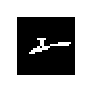
\includegraphics[width=1.1cm,height=1.1cm]{./figs/1_1133.eps}&
      	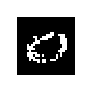
\includegraphics[width=1.1cm,height=1.1cm]{./figs/reconstructed_1.eps}\\
      (a) & (b) & (c) & (d)
\end{tabular}}
\centerline{\begin{tabular}{cccc}
      	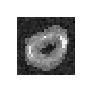
\includegraphics[width=1.1cm,height=1.1cm]{./figs/weight_1.eps} & 
      	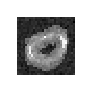
\includegraphics[width=1.1cm,height=1.1cm]{./figs/weight_2.eps} &
      	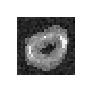
\includegraphics[width=1.1cm,height=1.1cm]{./figs/weight_3.eps}&
      	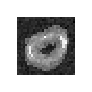
\includegraphics[width=1.1cm,height=1.1cm]{./figs/weight_4.eps}\\
      (e) & (f) & (g) & (h)
\end{tabular}}
\caption{(a) Dígito original `0'\ e (b) sua reconstrução, (c) dígito `1'\ e (d) sua reconstrução. Alguns pesos da RBM estão mostrados em (e)-(h).}
\label{f.weights}
\end{figure} 
}

\Sli{
\justifying Como podemos, então, utilizar RBMs para redução de dimensionalidade, aprendizado não supervisionado de características e ainda como pré-treinamento de redes neurais MLP?

\begin{itemize}
	\item Note que os valores presentes nas unidades escondidas $h_i\in\{0,1\}/$ ou ainda $P(h_i=1|\bm{v})$ podem ser utilizados como características e, quando $n<m$, temos uma redução do espaço original.
	\item Suponha que você tenha um conjunto grande de dados de treinamento, mas que somente uma pequena parte dele é rotulada. Você pode usar todo o conjunto de treinamento para o aprendizado de uma RBM (\textbf{não supervisionado}) e, em seguida, adicionar uma camada de saída à RBM e utilizar as imagens rotuladas para treinar uma MLP. Note que os pesos já estarão inicialmente aprendidos por meio do algoritmo de treinamento da RBM.
\end{itemize}
}

\SliT{Máquinas de Bolztmann Discriminativas}{
\justifying Como funcionam as RBMs no contexto de classificação? Para este tipo de fim, uma alternativa proposta corresponde às Máquinas de Boltzmann Restritas Discriminativas, do inglês \emph{Discriminative Restricted Boltzmann Machines} (DRBMs).\newline

\justifying De maneira geral, a ideia consiste em fazer uso do rótulo de cada amostra como entrada para a DRBM. A classificação é então realizada tentando ``reconstruir"\ o rótulo.
}

\Sli{
\justifying Temos, agora, uma unidade visível denominada $\bm{y}\in\{0,1\}^k$ e uma matriz de pesos $\bm{U}\in\mathbb{R}^{k\times n}$ que conecta $\bm{y}$ à camada escondida $\bm{h}$.\newline

\begin{figure}[!h]
\centerline{\begin{tabular}{cc}
      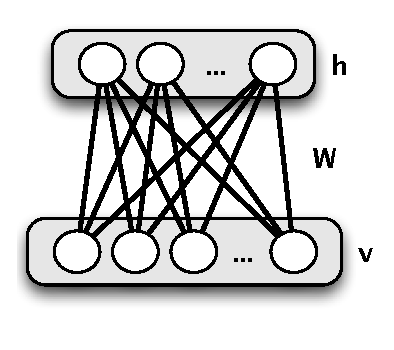
\includegraphics[width=4.1cm]{./figs/rbm2.eps} & 
      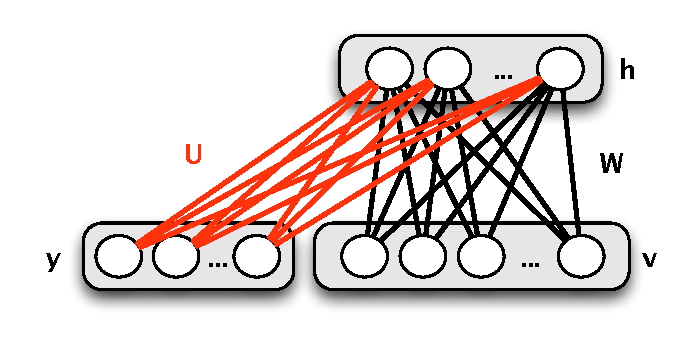
\includegraphics[width=7.5cm]{./figs/drbm.eps} \\
	(a) & (b)
  \end{tabular}}
  \caption{Arquitetura:~(a) RBM e~(b) DRBM.}
\label{f.rbm}
\end{figure}
}

\Sli{
\justifying Em uma DRBM, a camada $\bm{y}$ também assume valores binários para codificar a classe (\emph{one-hot encoding}). A probabilidade de \textbf{configuração conjunta} $P(\textbf{y},\textbf{v},\textbf{h})$ pode ser expressa da seguinte forma:

\begin{equation}
\label{e.joint_probability}
P(\textbf{y},\textbf{v},\textbf{h}) = \frac{e^{-E(\textbf{y},\textbf{v},\textbf{h})}}{\displaystyle\sum_{\textbf{y},\textbf{v},\textbf{h}}e^{-E(\textbf{y},\textbf{v},\textbf{h})}},
\end{equation}
em que a função de energia $E(\textbf{y},\textbf{v},\textbf{h})$ é dada por:

\begin{equation}
\label{e.energy}
E(\textbf{y},\textbf{v},\textbf{h})= - \sum_{i=1}^m\sum_{j=1}^nw_{ij}v_ih_j-\sum_{i=1}^ma_iv_i-\sum_{j=1}^nb_jh_j-\sum_{z=1}^kc_zy_z-\sum_{z=1}^k\sum_{j=1}^nu_{zj}h_jy_z,
\end{equation}
em que $\bm{c}\in\mathbb{R}^z$ corresponde à camada de bias da unidade de rótulos $\bm{y}$.
}

\Sli{
\justifying Assim sendo, a etapa de treinamento de uma RDBM objetiva encontrar o conjunto de parâmetros $\theta=(\textbf{W},\textbf{U},\textbf{a},\textbf{b},\textbf{c})$ que minimiza alguma critério de erro como, por exemplo, a MSE da unidade de rótulo reconstruída.\newline 

O procedimento de aprendizado por CD para encontrar $\theta$ consiste em calcular $P(\textbf{h}|\textbf{y},\textbf{v})$, o qual pode ser realizado para cada unidade $h_j$, $j=1,2,\ldots,n$ como segue:

\begin{equation}
\label{e.probh_yv}
P(h_j=1|\textbf{y},\textbf{v})=\phi\left(b_j+\sum_{z=1}^ku_{zj}y_z+\sum_{i=1}^mw_{ij}v_i\right),
\end{equation}
em que $\phi(\cdot)$ corresponde à função logística. 
}

\Sli{
\justifying Em seguida, podemos calcular a probabilidade condicional de obter $\textbf{v}$ dada cada camada escondida $\textbf{h}$ para cada unidade visível:

\begin{equation}
\label{e.probv_h}
P(v_i=1|\textbf{h})=\phi\left(a_i+\sum_{j=1}^nw_{ij}h_j\right),
\end{equation}
bem como a probabilidade de obter $\textbf{y}$ dada a unidade escondida $\textbf{h}$ para cada unidade da camada de rótulo, como segue:

\begin{equation}
\label{e.proby_h}
P(y_z=1|\textbf{h})=\frac{\exp\left(c_z+\displaystyle\sum_{j=1}^nU_{zj}h_j\right)}{\displaystyle\sum_{l=1}^k\exp\left(c_l+\displaystyle\sum_{j=1}^nU_{lj}h_j\right)}.
\end{equation}
}

\Sli{
\justifying O passo final da técnica CD consiste em calcular a Equação 20 mais uma vez para obtermos uma versão atualizada da camada escondida $\textbf{h}$. 

\begin{figure}[!h]
\centerline{\begin{tabular}{cc}
      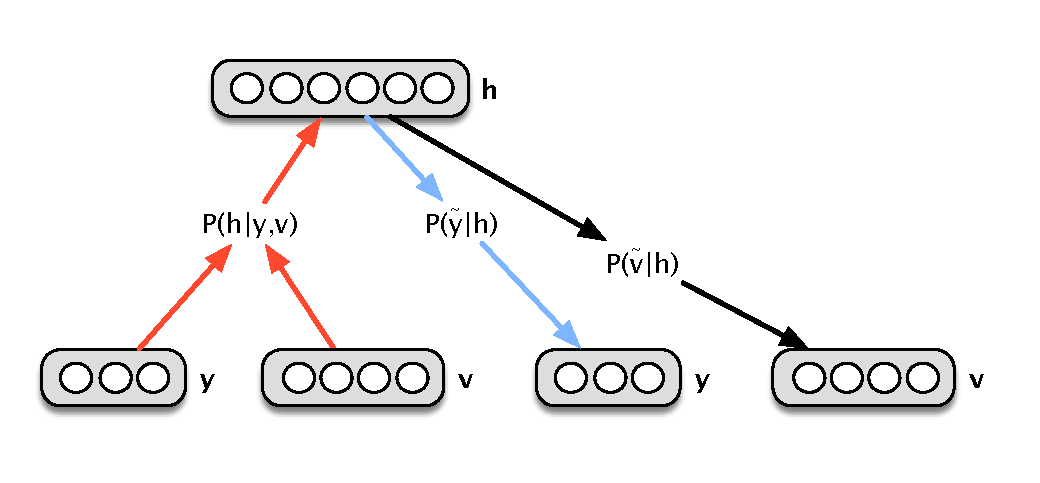
\includegraphics[width=7.7cm]{./figs/cd1.eps} & 
      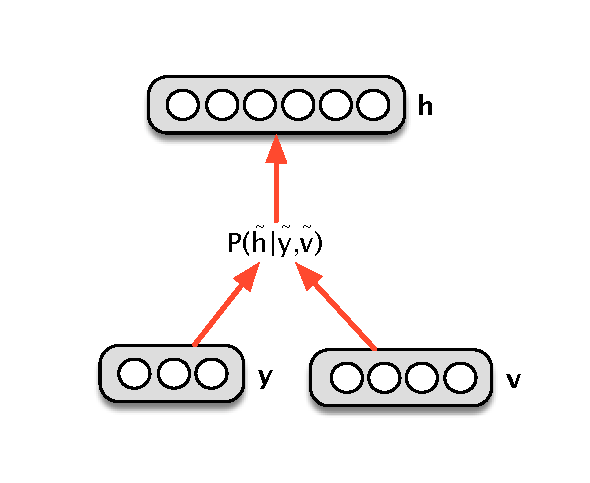
\includegraphics[width=4.3cm]{./figs/cd2.eps} \\
	(a) & (b)
  \end{tabular}}
  \caption{Aprendizado por CD:~(a) calcular as probabilidades condicionais para as unidades escondida (``vermelho"), rótulo (``azul") e visível (``preto"), e~(b) e calculando a probabilidade condicional da camada escondida mais uma vez.}
\label{f.cd}
\end{figure}
}

\Sli{
\justifying De maneira geral, o algoritmo de treinamento da DRBM consiste em estimar cada parâmetro em $\theta$ até algum critério de convergência ter sido atingido. Assim sendo, as seguintes equações de atualização podem ser aplicada no instante de tempo $t+1$:

\begin{equation}
\label{e.updateW}
 \textbf{W}^{t+1}=\textbf{W}^t+\underbrace{\eta(P(\textbf{h}|\textbf{y},\textbf{v})(\textbf{v})^T-P(\tilde{\textbf{h}}|\tilde{\textbf{y}},\tilde{\textbf{v}})(\tilde{\textbf{v}})^T)-\lambda\textbf{W}^t+\alpha\Delta\textbf{W}^{t-1}}_{=\Delta\textbf{W}^t},
\end{equation}

\begin{equation}
\label{e.updateU}
 \textbf{U}^{t+1}=\textbf{U}^t+\underbrace{\eta(P(\textbf{h}|\textbf{y},\textbf{v})(\textbf{y})^T-P(\tilde{\textbf{h}}|\tilde{\textbf{y}},\tilde{\textbf{v}})(\tilde{\textbf{y}})^T)-\lambda\textbf{U}^t+\alpha\Delta\textbf{U}^{t-1}}_{=\Delta\textbf{U}^t},
\end{equation}

\begin{equation}
\label{e.updatea}
\textbf{a}^{t+1}=\textbf{a}^t+\underbrace{\eta(\textbf{v}-\tilde{\textbf{v}})+\alpha\Delta \textbf{a}^{t-1}}_{=\Delta\textbf{a}^t},
\end{equation}

\begin{equation}
\label{e.updateb}
\textbf{b}^{t+1}=\textbf{b}^t+\underbrace{\eta(P(\textbf{h}|\textbf{y}\textbf{v})-P(\tilde{\textbf{h}}|\tilde{\textbf{y}},\tilde{\textbf{v}}))+\alpha\Delta \textbf{b}^{t-1}}_{=\Delta\textbf{b}^t},
\end{equation}
e

\begin{equation}
\label{e.updatec}
\textbf{c}^{t+1}=\textbf{c}^t+\underbrace{\eta(\textbf{y}-\tilde{\textbf{y}})+\alpha\Delta \textbf{c}^{t-1}}_{=\Delta\textbf{c}^t}.
\end{equation}

A etapa de classificação de uma DRBM pode ser realizada associando à uma dada amostra de teste $\textbf{x}$ a classe $e$, $e=1,2,\ldots,k$, que maximiza a equação abaixo:

\begin{equation}
p(y_e|\textbf{x})=\frac{\exp{-F(\textbf{x},y_e)}}{\displaystyle\sum_{y^\ast\in\{1,2,\ldots,k\}}\exp{-F(\textbf{x},\textbf{y}^\ast)}},
\end{equation}
em que $F(\textbf{x},y_e)$ corresponde à conhecida ``energia livre", que pode ser calculada como segue:

\begin{equation}
F(\textbf{x},\textbf{y})=c_e+\sum_{j=1}^n\varphi\left(\sum_{i=1}^mw_{ij}+U_{yj}+b_j)\right),
\end{equation}
em que $\varphi(z)$ corresponde à função \emph{softplus}, isto é, $\varphi(z)=\log(1+\exp(z))$. É importante lembrar que a unidade de rótulo $\textbf{y}$ é um vetor binário em que somente a posição $e$ está ligada quando $\textbf{y}$ representa a classe $e$.
}

\SliT{Redes de Crença em Profundidade}{
\justifying a
}

\end{document}